%% the main definitions for the report (KOMA-Script based)
\documentclass[11pt,a4paper,titlepage]{scrreprt}
\usepackage[T1]{fontenc}
\usepackage[utf8]{inputenc}
\usepackage[german,english]{babel}
%\usepackage{layouts}
\usepackage{graphicx}
\usepackage[round]{natbib}

\begin{document}

\selectlanguage{\german}

\title{{\Huge \bf MVC}\\[0.55em]{\LARGE Das Model-View-Controller-Konzept}}
\author{{\bf SE3 Team}\\Silvio Kunaschk}

\date{Juni 2009}
\maketitle

\begin{abstract}
Für die wahlobligatorische Vorlesung {\bf Software Engineering 3} von
Frau Professor Dr. Hauptmann, muß am Ende des Semesters in einer 
Gruppe von Studenten eine Belegarbeit zu einem gewählten Thema
angefertigt werden. Im SS09 wählte unsere Gruppe das Thema
{\bf Model-View-Controller-Konzept}.\\{\smallskip}

Die Zielstellung ist es, ein Software-System zu entwickeln zur Simulation
des MVC-Konzeptes. Unsere Gruppe hat sich dazu entschieden, das Konzept
anhand des {\itshape Model/View Programming Framework} von {\itshape Qt}
zu erläutern.\\{\smallskip}

Dieses Dokument beschreibt den allgemeinen Ansatz des 
Model-View-Controller-Konzeptes und erörtert dazu, anhand der Gesichtspunkte
eines Frameworks, die Umsetzung des Model-View-Controller Paradigma im
Qt Model/View~Programming~Framework.\\{\bigskip}

Die Gruppe besteht aus:
\begin{itemize}
\item Uwe Hausbrand
\item Tobias König
\item Silvio Kunaschk
\end{itemize}

\end{abstract}

\tableofcontents

\chapter{Allgemeine Betrachtungen}
In der Entwicklung von Software-Systemen haben sich\footnote{letztendlich} die Systeme durchgesetzt, 
welche mit Hilfe von graphischen Bedienoberflächen es dem Benutzer erlauben, das System
bzw. eine Anwendung interaktiv und nutzerfreundlich zu bedienen.

Dem Benutzer wird dadurch ein einfacher Zugriff auf das Software-System ermöglicht und
dabei geholfen, eine Anwendung zu verstehen und schneller und komfortabler damit zu arbeiten.

An der Akzeptanz und Verbreitung von Computer-Systemen in nahezu allen Bereichen der Industrie
und Wirtschaft und in letzter Zeit auch immer mehr im privaten gesellschaftlichen Bereich und
der Annahme, dass die meisten Anwender nur über rudimentäre
Informatikkenntnisse verfügen, aber trotzdem in der Lage sind mit Hilfe der graphischen
Benutzerschnittstelle die verschiedensten Aufgaben mit Software-Systemen einfach und effizient
zu lösen, kann man erkennen, welchen Stellenwert dieser Bestandteil von interaktiven
Software-Systemen besitzt.

Möchte man, dass sich sein Anwendungssystem bzw. Applikation durchsetzt, ist es heutzutage
unabdingbar eine ausgefeilte Benutzerschnittstelle mit zu implementieren, oder aber 
das System so zu entwickeln, dass dies von jeweiligen Fachleuten übernommen werden kann.

Spezifiziert man die Architektur eines interaktiven Software-Systems, muß man den funktionalen
Teil von der Bedienschnittstelle unabhängig halten. So können Änderungen an den Teilen
unabhängig voneinander durchgeführt werden, z.B. um die Benutzerschnittstelle an andere
Bedürfnisse anzupassen, ohne Auswirkungen auf den Funktionalen Teil des Systems.

Für diese grundlegende strukurelle Organisation interaktiver Software-Systeme wendet man
das Architekturmuster Model-View-Controller an.

\chapter{Das Model-View-Controller Muster}
\section{Das MVC Paradigma}
Das Model-View-Controller Muster teilt eine interaktive Anwendung in drei Komponenten auf.

\begin{figure}[h]
%\fbox{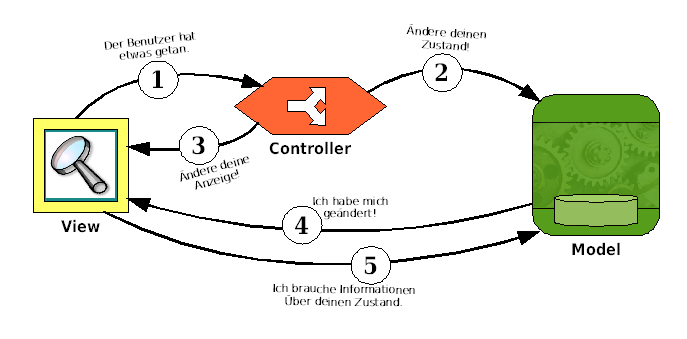
\includegraphics[width=14cm]{mvc-schema.png}}
% from: http://en.wikibooks.org/wiki/LaTeX/Importing_Graphics
%\includegraphics[trim = <trim from left> <from bottom> <from right> <from top>, clip, <other options>]{<image filename>}
%\includegraphics[trim = 10mm 80mm 20mm 5mm, clip, width=3cm]{chick}
\fbox{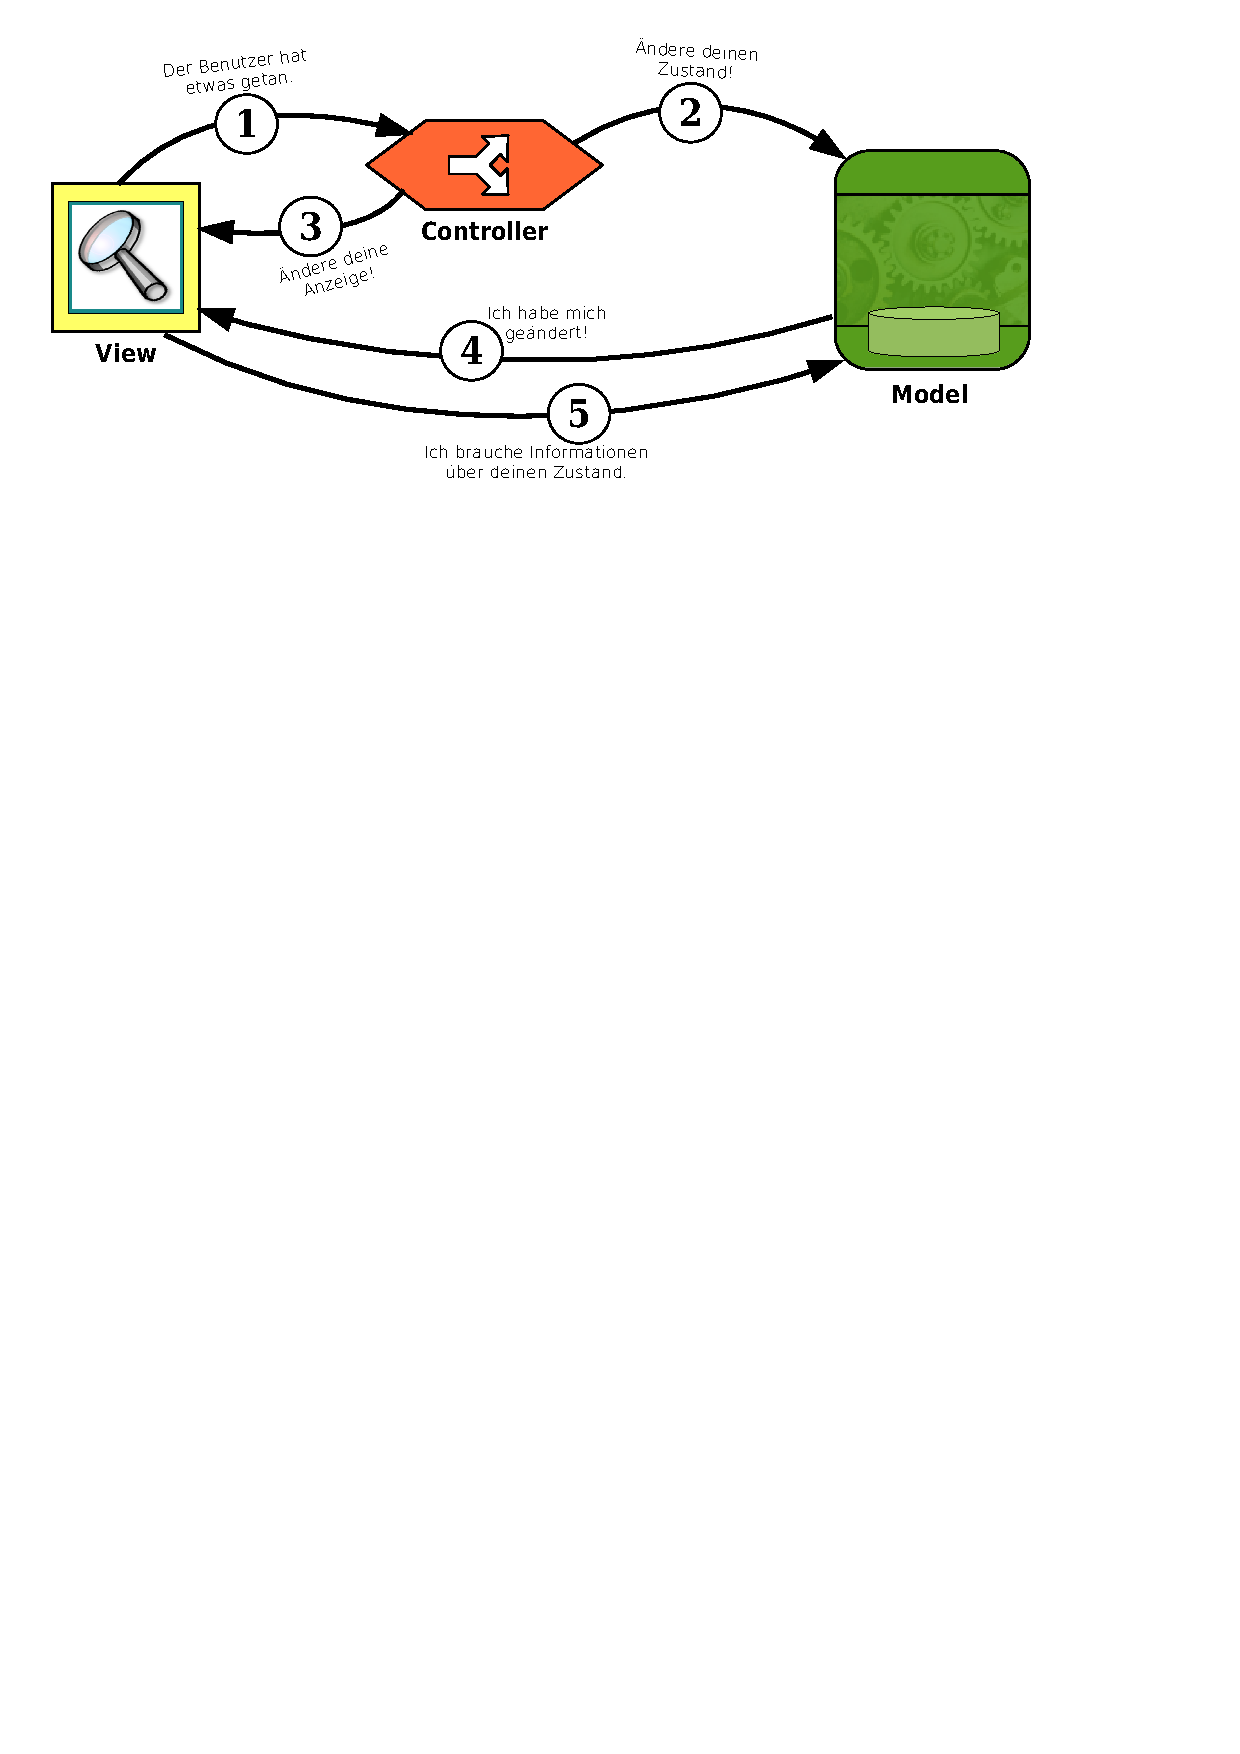
\includegraphics[trim = 0mm 207.7mm 28.6mm 0mm, clip, width=14cm]{mvc-schema.pdf}}
\caption{Die MVC Komponenten in Aktion}
\end{figure}

\begin{description}
\item[Model]
Das  Model stellt das Anwendungsobjekt dar. Es enthält die gesamte Daten, Zustands-
und Anwendungslogik. Es weiß nichts über Views und Controller, es bietet allerdings eine
Schnittstelle an, über die sein Zustand beeinflußt und abgerufen werden kann. Außerdem
kann es Benachrichtigungen über seine Zustandsänderungen an seine Beobachter senden.

\item[View]
Die View ist die Bildschirmrepräsentation des Anwendungsobjektes. Sie erhält den Zustand
und die Daten (normalerweise) direkt vom Model.

\item[Controller]
Der Controller bestimmt die Möglichkeiten, mit denen die Benutzungsschnittstelle auf
Benutzereingaben reagieren kann. Er nimmt die Eingaben des Benutzers entgegen und stellt
fest, was diese für das Model bedeuten. Er verarbeitet die Bedieneingaben.
\end{description}

Die View- und die Controllerkomponente beschreiben zusammen die Bedienschnittstelle.
Ein Benachrichtigungsmechanismus sichert die Konsistenz zwischen der Bedienschnittstelle
und dem Model.

Das MVC-Paradigma entkoppelt die Benutzungsschnittstellen der View vom Model. Dies
erhöht die Flexibilität und die Wiederverwendbarkeit.

\section{Das MVC etwas genauer betrachtet}
Schaut man beim Model-View-Controller etwas genauer hin, erkennt man, dass das MVC
ein Satz von Mustern ist, die in einem Entwurf zusammenarbeiten.\\
Es besteht eigentlich aus 3 Entwurfsmustern die hier aber nur kurz erläutert werden
sollen.

\subsection{Observer-Muster}
Das wichtigste Muster beim MVC-Konzept, auch für dessen Verständis, ist das Observer-Muster,
weshalb es hier jetzt genauer betrachtet wird.

\begin{description}
\item[Zweck]
Definiere eine 1-zu-n-Abhängigkeit, zwischen Objekten, so dass die Änderung des
Zustands eines Objektes dazu führt, dass alle abhängigen Objekte benachrichtigt
und automatisch aktualisiert werden. \citep[S. 287]{Riehle200407}
\end{description}

%% erzwinge das Anzeigen des Bildes genau an dieser Stelle
\enlargethispage{1cm}
\begin{figure}[h]
\fbox{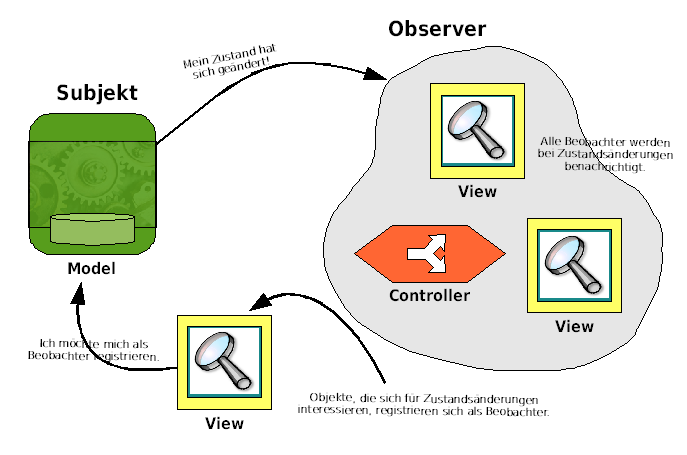
\includegraphics[width=14cm]{observer-schema.png}}
\caption{Das Observer-Muster in Aktion}
\end{figure}

Das Model nutzt das Observer-Muster, um View und Controller auf dem aktuellen
Stand über die letzten Zustandsänderungen zu halten.
Es macht das Model völlig unabhängig von View und Controller. So können für das gleiche
Model unterschiedliche, oder sogar mehrere Views auf einmal verwendet werden.

\begin{figure}[h]
\fbox{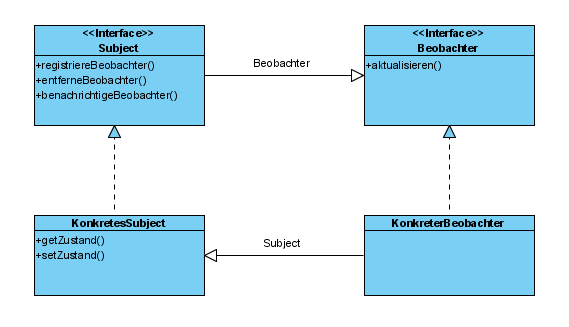
\includegraphics[width=14cm]{observer-kd.png}}
\caption{Das Observer-Muster Klassendiagramm}
\end{figure}

Ein Beobachter registriert sich beim Subjekt\footnote{beim MVC die View, und evtl.
auch der Controller, beim Model} und das Subjekt fügt es der Liste seiner Beobachter
hinzu. Ändert sich der Zustand des Subjektes, benachrichtigt es alle registrierten
Beobachter. Bei dem Benachrichtigungsvorgang wird vom Beobachter-Objekt die
aktualisieren-Methode aufgerufen. In diese Methode ist festgelegt, welche Daten
der Beobachter vom Subjekt benötigt und ruft diese über eine Schnittstelle beim
Subjekt ab.

\subsection{Strategy-Muster}
\begin{description}
\item[Zweck]
Definiere eine Familie von Algorithmen, kapsele jeden einzelnen und mache sie austauschbar.
Das Strategy-Muster ermöglicht es, den Algorithmus unabhängig von ihn nutzenden Klienten
zu variieren. \citep[S. 373]{Riehle200407}

\end{description}

Die View und der Controller implementieren das Strategy-Muster. Der Controller ist das
Verhalten der View und kann leicht gegen einen anderen Controller ausgetauscht werden,
wenn ein anderes Verhalten gewünscht wird.

Die View ist ein Objekt, das mit einer Strategie konfiguriert ist; der Controller
liefert diese Strategie. Die View ist nur für die Anzeige der Anwendung zuständig;
alle Entscheidungen über das Verhalten der Schnittstelle {\itshape delegiert} sie an
den Controller. Durch die Verwendung des Strategy-Muster bleibt die View vom
Model {\itshape entkoppelt}, denn der Controller ist ja bei der Bearbeitung der
Benutzeraktionen für die Interaktion mit dem Model zuständig. Die View weiß nicht
wie das vor sich geht.

\begin{figure}[h]
\fbox{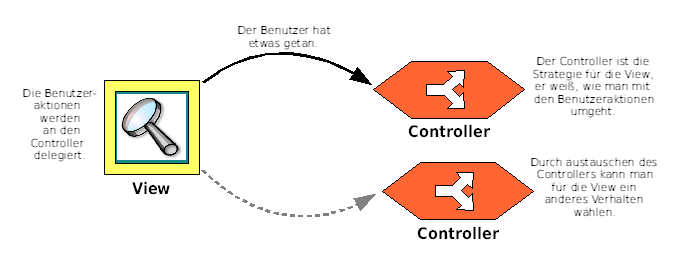
\includegraphics[width=14cm]{strategy-schema.png}}
\caption{Das Strategy-Muster in Aktion}
\end{figure}

Die View delegiert die Verarbeitung der Benutzeraktionen an den Controller. Der Controller
übersetzt die Eingaben des Benutzers in Aktionen auf dem Model.

\subsection{Composite-Muster}
Die View ist ein Kompositum aus GUI-Komponenten (Labels, Buttons, Texteingabefentern, usw. ).
Die oberste Komponente enthält andere Komponenten, die wiederum weitere Komponenten enthalten,
bis man beim Blattknoten angelangt ist. Sie verwendet dieses Muster intern, um die Bestandteile
der Anzeige zu verwalten.

\section{Nachteile von MVC}
Bei der Anwendung des MVC-Konzeptes sollte man sich durchaus auch bewußt darüber sein,
dass in bestimmten Fällen auch nachteilige Eigenschaften auftreten können, die nicht 
außer Acht gelassen werden sollten. \citep[vgl. S. 142]{Buschmann199801}

\begin{description}
\item[Größere Komplexität.]
Nicht immer ist die strikte Einhaltung der Model-View-Controller-Struktur die beste Art, eine
interaktive Anwendung zu entwickeln. Es kann sein das die Verwendung vom MVC die Komplexität
der Anwendung erhöht ohne den Zugewinn an Flexibilität.


\item[Potential für eine übermäßige Anzahl von Aktualisierungen.] Hat zum Beispiel eine
einfache Aktion des Anwenders viele Aktualisierungen zur Folge, sollte das Model unnötige
Benachrichtigungen über Änderungen auslassen. Eine View die gerade nicht sichtbar ist, braucht
nicht benachrichtigt zu werden.

\item[Enge Verbindung zwischen View- und Controllerkomponenten.] View und Controller sind
eigene, aber eng gekoppelte Komponenten, was deren jeweilige Wiederverwendung behindert.
Es ist unwahrscheinlich, dass eine View ohne ihre Controllerkomponente oder umgekehrt
verwendet wird.
\end{description}

\chapter{Framework}
\section{Ein kurzer Überblick}
An dieser Stelle werden kurz die wesentlichen Eigenschaften eines Frameworks aufgeführt,
um nachvollziehen zu können, unter welchen Aspekten das MVC-Muster angepasst wurde, um es
in das Qt-Framework zu integrieren.{\medskip}

Ein Framework besteht aus einer Menge von zusammenarbeitenden Klassen, die einen
wiederverwendbaren Entwurf für eine bestimmte Klasse von Software darstellen. Das
Framework bestimmt die Architektur der Anwendung. Es definiert:

\begin{itemize}
\item die Struktur im Großen
\item Unterteilung in Klassen und Objekte
\item die jeweiligen zentralen Zuständigkeiten
\item die Zusammenarbeit der Klassen und Objekte sowie den Kontrollfluß
\end{itemize}

Ein Framework legt diese Entwurfsparameter im voraus fest, so dass der Entwickler
sich auf die spezifischen Details seiner Anwendung konzentrieren kann.
Verwendet man ein Framework, schreibt man den Code, der vom Framework gerufen wird.
Dies wird erreicht indem man Operationen mit bestimmten Namen und Aufrufkonventionen
schreiben muß. Dies reduziert die zu treffenden Entwurfsentscheidungen. Diese sind
bereits von anderen getroffen worden.

Speziell bei GUI-Frameworks ermöglicht diese Vorgehensweise ein sehr viel schnelleres
Entwickeln von Anwendungen\footnote{in diesem Fall von den View-Komponenten
der Anwendung}. Diese haben eine ähnliche Struktur und sind einfacher Wiederverwendbar.
Auf der einen Seite schränkt dies die Kreativität ein, aber man erhält Komponenten 
in denen Erfahrung steckt und die schon erprobt sind. Dem Benutzer der Anwendung sind
diese Verhaltensweisen in der Regel schon bekannt.

\chapter{Model/View Programmierung mit dem Framework von Qt}
\section{Was ist Qt?}
Qt ist das de facto Standard C++ Framework für ein sehr schnelles Entwickeln von
Cross-Platform-Software. Zusätzlich zu einer sehr Umfangreichen C++ Klassenbibliothek
enthält Qt Werkzeuge, die das Schreiben von Anwendungen erleichtern und
beschleunigen.

Qt enthält eine große Menge von Widgets, welche Standard GUI-Funktionalität zur
Verfügung stellen. Qt ist ein weltweit verwendetes und ausgereiftes C++ Framework.

Neben den vielen kommerziellen Verwendungen von Qt, ist die Open Source Edition
von Qt die Grundlage von KDE, der Linux Desktop Umgebung.

\section{Item Views}
Qt`s Item-View-Widgets stellen Standard GUI-Bedienungselemnte zur Verfügung, für die
Anzeige und Modifizierung großer Datenmengen. Das zugrundeliegende Model/View Framework
entkoppelt die Art der Datenspeicherung von der Art ihrer Repräsentation dem Anwender
gegenüber. Weitere Vorteile sind mehrfache Datennutzung, Sortierung und Filterung,
mehrfache Views und Datenrepräsentationen auf den selben Daten.

Wenn man Anwendungen schreibt, die große Mengen an Daten verarbeiten, werden die
Entwickler Item-View-Widgets verwenden, um die Daten schnell und effizient anzuzeigen.
Die Standard Item Views vieler moderner GUI-Frameworks enthalten Listen-Ansichten,
Tree-Views mit hierarchisch angeordneten Listen und Table-Views, wie man sie 
beispielsweise in Tabellenkalkulationen finden kann.

Qt`s Item View Klassen gibt es in 2 verschiedenen Formen: als klassische Item-View-Widgets
und als Model/View Komponenten. Klassische Item Views, wie {\itshape QListWidget}, 
{\itshape QTableWidget} und {\itshape QTreeWidget}, sind eigenständige Views, welche Items
verwalten, die explizit vom Entwickler angelegt werden.

%% erzwinge das Anzeigen des Bildes genau an dieser Stelle
\enlargethispage{1cm}
\begin{figure}[h]
\fbox{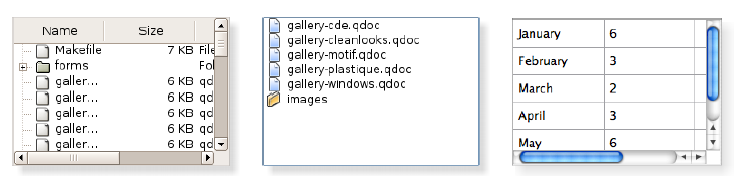
\includegraphics[width=14cm]{qt-widgets.png}}
\caption{Die Standard Item Views von Qt für Tree-, List- und Tableviews}
\end{figure}

{\itshape QListView}, {\itshape QTableView} und {\itshape QTreeView} sind die äquivalenten
Model/View Komponenten zu den klassischen Item Views. Diese Komponenten bieten eine
einfache und saubere, Komponenten-orientierte Art die Datenmengen zu verwalten.

\section{Das Model/View Framework}
Das Model/View Framework, welches von Qt bereitgestellt wird, ist eine Variante des
Model-View-Controller-Konzeptes, welche speziell für Qt`s Item Views angepasst wurde.
Dabei werden Models verwendet, um Daten anderen Komponenten zur Verfügung zu stellen,
Views präsentieren sie dem Anwender und Delegates behandeln die Aspekte der
Rendering- und Bearbeitungsprozesse.

Models sind Wrapper um Datenquellen, welche konform zum Standardinterface sind, welches
von {\itshape QAbstractItemModel} angeboten wird. Dieses Interface ermöglicht es Widgets,
welche von {\itshape QAbstractItemView} abgeleitet wurden, auf Daten zuzugreifen, welche 
über das Model zur Verfügung gestellt werden, ungeachtet welcher Natur\footnote{z.B.
aus SQL-Datenbanken, XML-Daten, Textdateien, ...} die Original Datenquelle ist.
Die Trennung zwischen den Daten und ihrer Darstellung, welche dieser Ansatz ermöglicht,
bietet eine ganze Reihe von Vorteilen gegenüber den klassischen Item Views:
\begin{itemize}
\item Durch die Verwendung eines Standard-Interface für den Datenzugriff der Models,
können diese separat von anderen Komponenten entwickelt und bei Bedarf ersetzt werden.
\item Daten, welche über Models erhalten werden, können zwischen mehreren Views geteilt werden.
Dadurch wird es der Anwendung ermöglicht, verschiedenste Darstellungsformen der selben Daten
durch mehrere Views anzubieten.
\item Markierte Daten können zwischen den Views geteilt oder getrennt verwaltet werden, je
nachdem was vom Anwender gewünscht wird.
\item Für die Standard-Views List, Tree und Table, wird das meiste des Renderingvorganges von
Delegates ausgeführt. Das erleichtert das Anpassen der Views für die meisten Zwecke, ohne
viel neuen Code zu schreiben.
\item Durch die Verwendung von {\itshape Proxy Models} können Daten, die von Models angeboten
werden, transformiert werden, bevor sie der View zur Verfügung gestellt werden. Dies ermöglicht
es Sortierung und Filterung der Anwendung hinzuzufügen, die zwischen mehreren Views verwendet
werden kann.
\end{itemize}

\section{Die Model/View Architektur}
Die Model/View Architektur resultiert aus der Kombination der View und des Controllers,
des Model-View-Controller-Konzeptes, in einer Komponente. Dies trennt immer noch die
Datenhaltung von der Art ihrer Präsentation, aber ermöglicht einen Framework basierten
Ansatz auf der selben Grundlage. Um flexibel auf Benutzereingaben zu reagieren, wird das
Konzept der {\itshape Delegates} eingeführt. Der Vorteil bei der Verwendung von Delegates
in diesem Framework besteht darin, dass es erlaubt, die Art und Weise des Renderings und Editieren
von Daten individuell anzupassen.{\medskip}

\begin{figure}[h]
\begin{center}
\fbox{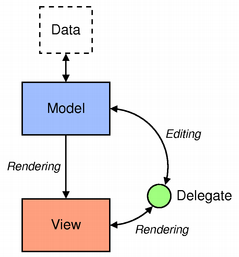
\includegraphics[width=5cm]{modelview-overview.png}}
\caption{Die Model/View Architektur}
\end{center}
\end{figure}

\begin{description}
\item[Model]
Das Model kommuniziert mit einer Datenquelle und bietet ein Interface für den Zugriff
der anderen Komponenten an. Die Art der Kommunikation\footnote{zwischen Model und
Datenquelle} hängt von der Art der verwendeten Datenquelle ab.
\item[View]
Die View bekommt {\itshape Model-Indizies} vom Model, welche die Daten-Items referenzieren.
Übergibt die View dem Model Model-Indizies, so erhält sie die Daten-Items von der Datenquelle.
\item[Delegate]
In Standardviews rendert ein Delegate die Daten-Items. Wird ein Item bearbeitet,
kommuniziert das Delegate direkt mit dem Model über den Model-Index.
\end{description}

Generell kann man die Model/View-Klassen in diese drei, wie oben beschrieben, Gruppen
einteilen: Models, Views und Delegates. Jede dieser Komponenten wird von {\itshape abstrakten
Klassen} definiert, welche die gemeinsamen Interfaces anbieten und manchen Fällen die
standardmäßige Implementierung von Features.

Model, Views und Delegates kommunizieren miteinander unter der Verwendung von 
{\itshape Signals} und {\itshape Slots}\footnote{Der Signal und Slot Mechanismus 
ist im Qt Framework für die Kommunikation zwischen Objekten zuständig}:
\begin{itemize}
\item Signals vom Model informieren die View über Änderungen der Daten in der Datenquelle
\item Signals von der View bieten Informationen über die Benutzeraktion auf den angezeigten
Daten-Items
\item Signals vom Delegate werden während der Dateneditierung verwendet, um Model und
View über den Status der Editierung zu informieren
\end{itemize}

\subsection{Models}
Alle Item-Models basieren auf der {\itshape QAbstractItemModel} Klasse. Diese definiert ein
Interface, über welches von Views und Delegates aus auf die Daten zugegriffen werden kann.
Die Daten selbst müssen nicht innerhalb des Models gespeichert werden. Sie werden über andere
Datenstrukturen oder Quellen verwaltet, einer Datei, eine Datenbank oder irgendetwas anderes.

\subsection{Views}
Vollständige Implementierungen werden für die Views {\itshape QListView}, {\itshape QTableView} und
{\itshape QTreeView} zur Verfügung gestellt. Jede dieser Klassen basiert auf der abstrakten
Basisklasse {\itshape QAbstractItemView}. Obwohl diese Klassen schon fertig zur Benutzung sind,
können sie weiter angepasst werden.

\subsection{Delegates}
{\itshape QAbstractItemDelegate} ist die abstrakte Basisklasse für Delegates im Model/View
Framework. Eine Standardimplementierung wird von {\itshape QStyledItemDelegate} angeboten und
diese wird von den Qt-Standardviews verwendet.

\subsection{Sortieren}
Es gibt einen alternativen Ansatz um Daten in der Model/View Architektur zu sortieren. Bietet
ein Model keine standardmäßigen Interfaces für Sortierung an\footnote{um beispielsweise Listen
zu sortieren, \dots}, kann man mit der Hilfe von {\itshape Proxy Models} die Struktur der Daten
des Models vor ihrer Darstellung in der View transformieren.

\newpage
% "leeres" Zitieren um alle Angabe aus dem Literaturverzeichnis als Quellen auszugeben
\nocite{*}
\addcontentsline{toc}{chapter}{Literaturverzeichnis}
\bibliography{mvc-literatur}{}
\bibliographystyle{plain}

\end{document}
